\documentclass[oneside]{book}

\setcounter{tocdepth}{1}
\setcounter{secnumdepth}{3}

\usepackage[toc,page]{appendix}
\usepackage{hyperref}
\usepackage[utf8]{inputenc}
\usepackage{graphicx} % Required for the inclusion of images
\usepackage{amsmath} % Required for some math elements 
\usepackage[utf8]{inputenc}
\usepackage[english]{babel}
\newtheorem{theorem}{Theorem}
\newtheorem{corollary}{Corollary}[theorem]
\newtheorem{lemma}[theorem]{Lemma}
\usepackage{listings}
\usepackage{pdfpages}
\usepackage{amssymb}
\usepackage{pdflscape}

\begin{document}

\begin{titlepage}
	\centering
	
\includegraphics[width=0.60\textwidth]{../../logo/UoN_Primary_Logo_RGB.png}\par\vspace{1cm}
	\vspace{1.5cm}
	{\huge\bfseries The Pure Functional and \\ Object-Oriented Paradigm \\ in Agent-Based Simulation \par}
	\vspace{2cm}
	{\Large\itshape jonathan.thaler@nottingham.ac.uk \par}
	\vfill
	
	\vfill

	{\large \today\par}
\end{titlepage}

\cleardoublepage

\section*{Abstract}
This study we compares the object oriented and pure functional programming paradigms to implement Agent-Based Simulation. Due to fundamentally different concepts both propagate fundamental different approaches in implementing ABS. In this document we seek to precisely identify these fundamental differences, compare them and also look into general benefits and drawbacks of each approach.

\clearpage
\tableofcontents
\clearpage

\section{Introduction}
There exists a large number of simulation packages which allow the convenient creation of System Dynamics simulations by straight-forward visual diagram creation. One simply creates stocks and flows, connects them, specifies the flow-rates and initial parameters and then runs the model. An example for such a visual diagram creation in the simulation package AnyLogic can be seen in Figure \ref{fig:sir_stockflow_diagram}.

\begin{figure}
	\centering
	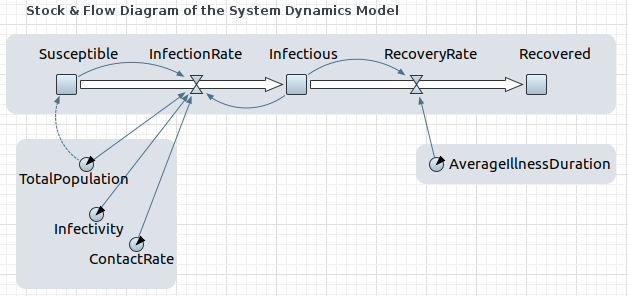
\includegraphics[width=.5\textwidth, angle=0]{./fig/SIR_SD_STOCKFLOW_DIAGRAMM.png}
	\caption{Visual System Dynamics Diagram of the SIR model in AnyLogic Personal Learning Edition 8.3.1.}
	\label{fig:sir_stockflow_diagram}
\end{figure}

Still, implementing System Dynamics directly in code is not as straight forward and involves numerical integration which can be quite tricky to get right. Thus, the aim of this paper is to look into how System Dynamics models can be implemented in code correctly without the use of a simulation package. We use the well known SIR model \cite{kermack_contribution_1927} from epidemiology to demonstrate our approach.

Our language of choice is Haskell because it emphasises a declarative programming style in which one describes \textit{what} instead of \textit{how} to compute. Further it allows to rule out interference with non-deterministic influences or side-effects already at compile-time. This is of fundamental importance for System Dynamics because it behaves completely deterministic and involves no stochastics or non-determinism whatsoever. Also, we make use of Functional Reactive Programming which allows to express continuous-time systems in a functional way. 

We show that by this approach we can arrive at correct-by-construction implementations of System Dynamic models. This means that the correctness of the code is obvious because we have closed the gap between the model specification and its implementation. Thus, the contribution of the paper is the demonstration of how to implement correct-by-construction System Dynamics simulations using Haskell and Functional Reactive Programming.

\section{Pure Functional Programming}
\label{sec:background_fp}
To be able to understand the challenges of pure functional ABS as well as the solutions and concepts developed in this thesis, in this section we give a short introduction to functional programming, with an overview of its concepts and advanced features. As it is obviously beyond the focus of a thesis to give a full treatment of such a complex topic, we refer to additional literature and references for further discussions where appropriate.

Functional programming is called \textit{functional} because it makes functions the main concept of programming, promoting them to first-class citizens. This means that functions can be assigned to variables, they can be passed as arguments to other functions and they can be constructed as return values from functions. The roots of functional programming lie in Lambda Calculus which was first described by Alonzo Church \cite{church_unsolvable_1936}. This is a fundamentally different approach to computing than imperative programming (including established object-orientation), the roots of which lie in the Turing Machine \cite{turing_computable_1937}. Rather than describing \textit{how} something is computed as in the more operational approach of the Turing Machine, due to the more \textit{declarative} nature of Lambda Calculus, code in functional programming describes \textit{what} is computed.

In \cite{maclennan_functional_1990} the author defines functional programming as a methodology attributing the following properties to it: programming without the assignment-operator, allowing for higher levels of abstraction, allowing to develop executable specifications and prototype implementations, connected to computer science theory, performing algebraic reasoning. Further, the author makes the subtle distinction between \textit{applicative} and \textit{functional} programming. Applicative programming can be understood as applying values to functions where one deals with pure expressions. In those expressions the value is independent from the evaluation order, also known as referential transparency. This means that such functions have no side effects and thus the outcome of their execution does not depend on the history or context of the system. Additionally, inputs and effects to an operation are obvious from the written form.

Applicative programming is not necessarily unique to the functional programming paradigm but can be emulated in an imperative language like C as well. Functional programming is then defined by \cite{maclennan_functional_1990} as applicative programming with \textit{higher-order} functions. These are functions which operate themselves on functions: they can take functions as arguments, construct new functions and return them as values. This is in stark contrast to first-order functions, as used in applicative or imperative programming, which just operate on data alone. Higher-order functions allow the capturing of frequently recurring patterns in functional programming in the same way that imperative languages captured patterns like \texttt{goto}, \texttt{while-do}, \texttt{if-then-else}, \texttt{for}. Common patterns in functional programming are (amongst others) the \texttt{map}, \texttt{fold}, \texttt{zip} functions. So, functional programming is not really possible in the same way as in classic imperative languages like C, as it is not possible to construct new functions and return them as results from functions. Object-oriented languages like Java provide mechanisms allowing us to partially work around this limitation but are still far from \textit{pure} functional programming.

The equivalence in functional programming to the semicolon (;) operator of imperative programming, that allows us to compose imperative statements, is function composition. Function composition has no side effects, as opposed to the imperative semicolon operator, which simply composes destructive assignment statements executed after another, resulting in side effects.
At the heart of modern functional programming is monadic programming which is polymorphic function composition. One can implement a user-defined function composition by running code in between function composition - this code, of course, depends on the type of the Monad one runs in. This allows for emulating all kinds of effectful programming in an imperative style within a pure functional language (see Section \ref{sec:purity_sideeffects} below). Although it might seem strange following an imperative style in a pure functional language, some problems are inherently imperative in the way that computations need to be executed in a given sequence exhibiting some effects. In addition, a pure functional language needs to have some way to deal with effects, otherwise it would never be able to interact with the outside world and would be practically useless. The real benefit of monadic programming is that it is explicit about side effects and allows only effects which are fixed by the type of the Monad - the side effects which are possible are determined statically during compile time by the type system. Some general patterns can be extracted for example a \texttt{map}, \texttt{zip}, \texttt{fold} over Monads which results in effect-polymorphic behaviour. %this is the meaning when one says that a language is polymorphic in its side effects.

\subsection{Language of choice}
In our research we are using the \textit{pure} functional programming language Haskell. The paper \cite{hudak_history_2007} gives a comprehensive overview over the history of the language, how it developed and its features. The reasons for choosing Haskell are as follows:

\begin{itemize}
	\item Rich feature-set - it has all the fundamental concepts of the pure functional programming paradigm included, of which the most important ones are explained below. Moreover, Haskell has influenced a large number of languages, underlining its importance and influence in programming language design.
	
	\item Real-world applications - the strength of Haskell has been proven through a vast amount of highly diverse real-world applications \cite{hudak_history_2007, hudak_haskell_1994}. It is applicable to a number of real-world problems \cite{osullivan_real_2008} and has a large number of libraries available \cite{haskell_applications}.
	
	\item Modern - Haskell is constantly evolving through its community and adapts to keep up with the fast-paced changes in the field of computer science. Additionally, the community is the main source of high-quality libraries.
	
	\item Highly advanced type system - Haskell has a strong static type system, which catches all type errors at compile time and does not allow for bypassing the type system (unless \texttt{coerce} or other cheating functions like \texttt{unsafePerformIO} are used). In addition, Haskell is a \textit{pure} functional language and in our research it is absolutely paramount, that we focus on \textit{pure} functional ABS, which avoids any \texttt{IO} type under all circumstances. This property is enabled by the advanced type system and its strong static nature.
\end{itemize}

A highly compelling example motivating the benefits of pure functional programming is the report \cite{hudak_haskell_1994}. Where, in a prototyping contest of DARPA the Haskell prototype was by far the shortest, with 85 lines of code (LoC), as compared to the C++ solution with 1105 LoC. The remarkable thing is that the jury mistook the Haskell code as specification because its approach was to implement a small embedded domain specific language (EDSL) to solve the problem. This is a perfect proof as to how close an EDSL can get to a specification. When implementing an EDSL, one develops types and functions in a host language (embed) in a way where they can be combined. The combination of these primitives then looks like a language specific to a given domain. The ease of development of EDSLs in pure functional programming is also proof of the superior extensibility and composability of pure functional languages over object-orientation and is definitely one of its major strengths. The classic paper \cite{henderson_functional_1982} shows a wonderful way of constructing an EDSL to denotationally construct a picture reminiscent of the works of M.C.Escher. A major strength of developing an EDSL is that one can formally reason about it and do formal verification. A nice introduction about how to do reasoning in Haskell is given in \cite{hutton_tutorial_1999}.

For an excellent and widely used introduction to programming in Haskell we refer to \cite{hutton_programming_2016}. Other, more exhaustive books on learning Haskell are \cite{allen_haskell_2016, lipovaca_learn_2011}. For an introduction to programming with the Lambda-Calculus we can refer to \cite{michaelson_introduction_2011}. For a more general discussion of functional programming we refer to \cite{hudak_history_2007,hughes_why_1989,maclennan_functional_1990}.

\subsection{An Example}
Consider the factorial function in Haskell:
\begin{HaskellCode}
factorial :: Integer -> Integer
factorial 0 = 1
factorial n = n * factorial (n-1)
\end{HaskellCode}

When looking at this function, the following can be identified: 
\begin{enumerate}
	\item Declarative - describe \textit{what} the factorial function is, rather than how to compute it. This fact is supported by \textit{pattern matching} which allows providing multiple equations for the same function, matching on its input. 
	
	\item Immutable Data - in functional programming there are no mutable variables, after a variable is assigned, it cannot change its contents. This also means that there is no destructive assignment operator that can reassign values to a variable. To change values, recursion is employed.

	\item Recursion - the function calls itself with a structurally smaller argument and will eventually reach the base case of 0. Recursion is the very meat of functional programming because it is the only way to implement loops in this paradigm due to immutable data.
	
	\item Static Types - the first line indicates the name and the type of the function. In this case the function takes one Integer as input and returns an Integer as the output. Types are static in Haskell, which means that there can be no type errors at run time. For example it is not supported by this kind of type system to implicitly cast one type into another.

	\item Explicit Input and Output - all data which are required and produced by the function have to be explicitly passed in and out of it. No global mutable data exists whatsoever and data flow is always explicit.
	
	\item Referential Transparency - calling this function with the same argument will \textit{always} lead to the same result. Meaning one can replace this function by its value. Consequently, when implementing this function one cannot read from a file or open a connection to a server. This is also known as \textit{purity} and is indicated in Haskell in the types which means that it is also guaranteed by the compiler.
\end{enumerate}

It may seem that one runs into efficiency problems in Haskell when using algorithms which are implemented in imperative languages through mutable data, which allows in-place update of memory. The seminal work of \cite{okasaki_purely_1999} shows that when approaching this problem with a functional mindset, this issue will not necessarily be the case. The author presents functional data structures which are asymptotically as efficient as the best imperative implementations and discusses the estimation of the complexity of lazy programs.

\subsection{Purity and Side Effects}
\label{sec:purity_sideeffects}
One of the fundamental strengths of Haskell is its way of dealing with side effects in functions. A function with side effects has observable interactions with some state outside of its explicit scope. Therefore, its behaviour depends on the history of the system which means that it loses its referential transparency character, which makes understanding and debugging much harder. Possible examples of side effects are (amongst others): modifying a variable, awaiting an input from the keyboard, reading or writing to a file, opening a connection to a server, drawing random numbers.

Obviously, to write real-world programs which interact with the outside world requires side effects. Haskell allows for indicating in the \textit{type} of a function that it does, or does \textit{not} have side effects. What is more, there is a broad range of different effect types available, to restrict the possible effects a function can have to only the required type. This is checked by the compiler, which means that code which tries to read from a file in a function, when only allowing for drawing random numbers, will fail to compile.

A function without any side effect type is called \textit{pure}, and the \texttt{factorial} function discussed above is indeed pure. Below we give the \texttt{queryUser} function as an example of a function which is not pure. It constructs a computation, which when executed, asks the user for its user name and compares it with a given user configuration. In the event that the user name matches, it returns \texttt{True}, and \texttt{False} otherwise after printing a corresponding message. The effect type of the function is \texttt{IO}, which allows all kind of input-output related side effects like reading and writing a file, creating threads, writing to the standard output, reading from the keyboard, opening network connections and modifying mutable references.

\begin{HaskellCode}
queryUser :: String -> IO Bool
queryUser username = do
  -- print text to console
  putStr "Type in user-name: "
  -- wait for user-input
  str <- getLine
  -- check if input matches user-name
  if str == username
    then do
      putStrLn "Welcome!"			
      return True
    else do
      putStrLn "Wrong user-name!"
      return False
\end{HaskellCode}

What seems striking is that this looks very much like imperative code, which is no coincidence, but rather very much intentional. When we are dealing with side effects, ordering becomes important. Thus, Haskell introduced the so-called \textit{do} notation which emulates an imperative style of programming. Whereas, in imperative programming languages like C, instructions are chained or composed together using the semicolon (;) operator, in functional programming this is done using function composition. That is, feeding the output of a function directly into the next function. The machinery behind the \textit{do} notation does exactly this and desugars this imperative-style code into function compositions which run custom code between each line, depending on the type of effect the computation runs in. This approach of function composition with custom code in between each function allows to emulate a broad range of imperative-style effects, including the above-mentioned ones.

Although it might seem very restrictive at first, we get a number of benefits from making the type of effects we can use in a function explicit. First, we can restrict the side effects a function can have to a very specific type which is guaranteed at compile time. This means we can have much stronger guarantees about our program and the absence of potential errors immediately at compile time. Second, because running effects themselves is \textit{pure}, we can execute functions with effects in a very controlled way by making the context of the effect explicit in the parameters to the effect execution. This allows for a much easier approach to isolated testing because the history of the system is made explicit. 

\subsubsection{Monads}
Haskell implements its way of dealing with side effects using the concept of \textit{Monads}. It is important to understand that Monads are implemented directly in Haskell, which means that effects (with the exception of \texttt{IO} Monad) are implemented in terms of Haskell and not built into the runtime. To better understand how Haskell implements its concept of side effects with Monads, in this section, we briefly give an overview of what Monads are, how they are defined in Haskell and how they are used to facilitate effectful programming in a pure functional way. As this is a vast and complex topic, we can only scratch the surface here, consequently for a more technical, in-depth discussion we refer to \cite{jones_tackling_2002,moggi_computational_1989,wadler_essence_1992,wadler_monads_1995,wadler_how_1997}.

A Monad is an algebraic structure from the field of Category Theory. Moggi \cite{moggi_computational_1989} realised that Monads can be used to structure computation and later, Wadler \cite{wadler_monads_1995,wadler_how_1997} realised that Monads can be used as a way to achieve effectful computation in pure functional programming. 

Without going into the mathematical details, we give the definition of Monads in Haskell. Informally speaking, in Haskell, a Monad is both an Applicative and a Functor, which provides the operation \textit{return} and \textit{bind}. The according type class is:

\begin{HaskellCode}
-- Monad type class
-- Applicative and Functor omitted for clarity
class Applicative m => Monad m where
  return :: a -> m a
  -- bind, in Haskell >>= is used
  (>>=) :: m a -> (a -> m b) -> m b
\end{HaskellCode}

%-- Applicative type class
%-- Allows composing functions which map over values with structure.
%class Functor f => Applicative f where
%  pure  :: a -> f a
%  (<*>) :: f (a -> b) -> f a -> f b
%
%-- Functor type class
%-- Allows mapping between values with some structure.
%class Functor f where
%  fmap :: (a -> b) -> f a -> f b

\texttt{return} lifts a pure value into a Monad. \texttt{bind (>>=)} allows to sequence computations, feeding the output \texttt{a} of the first computation into a continuation, which returns a new computation in the same Monad \texttt{m} but with a possibly different return type \texttt{b}. Interestingly, with this interface it becomes possible to implement a wide range of pure, deterministic effects. As already mentioned above, in between lines of the \textit{do} notation runs custom code. This is achieved which the \texttt{bind (>>=)} method. The \texttt{return}, also seen above in the example, lifts a pure value, in the example a \texttt{Boolean} value, into a monadic value.

Obviously, the Monad type class only defines the interface required for a Monad but no actual implementations. There are a number of different Monad implementations, providing different types of side effects:

\begin{itemize}
	\item \texttt{Reader} uses partial function application to implement reading from an environment;
	\item \texttt{Writer} uses a monoid type to implement writing to a \textit{monoid} environment;
	\item \texttt{State} uses functions and closures to implement reading and writing shared state of a given type;
	\item \texttt{Rand} uses a \texttt{State} Monad to implement a random number stream;
	\item \texttt{[] (List)} forms also a Monad and implements non-deterministic programming.
\end{itemize}

To better understand how a Monad is implemented, we show the implementation of the \texttt{Maybe} Monad, which allows programming with failure. The \texttt{Maybe} type itself is straightforward and provides some kind of optional value, where a computation can either return \texttt{Just} some value or \texttt{Nothing}:

\begin{HaskellCode}
data Maybe a = Nothing | Just a
\end{HaskellCode}

Interestingly, \texttt{Maybe} forms a Monad. It allows us to write imperative-style code with the option of failure but saves us from handling each failure individually. Here is the implementation:

\begin{HaskellCode}
-- Instance of Maybe Monad.
-- Type definitions of methods provided for clarification
instance Monad Maybe where
  return :: a -> Maybe a
  return = Just
  
  (>>=) :: Maybe a -> (a -> Maybe b) -> Maybe b
  (>>=) Nothing _  = Nothing
  (>>=) (Just a) f = f a 
\end{HaskellCode}

\texttt{return} simply lifts a pure value \texttt{a} into a \texttt{Just} value, applying the data constructor \texttt{Just}. \texttt{bind (>>=)} performs case analysis: if \texttt{Maybe a} is Nothing, the it will propagate \texttt{Nothing}, otherwise it will use \texttt{a} with the continuation \texttt{f}, to return the next computation \texttt{Maybe b}.

\medskip

It is important to understand that the code fragments of effectful computations are in fact  made up of enclosing lambda expressions, with the \textit{do} notation being a syntactic sugared version. Thus functions which have an effect in their type can be seen as \textit{pure} functions, which are referentially transparent and return such a fragment. This fragment, often called \textit{action}, results in an effect and a result when executed. We have to distinguish between the execution of pure effects like \texttt{Rand}, \texttt{Read}, \texttt{Write}, \texttt{State} and the impure effect of \texttt{IO}. Pure effects are executed using special runner functions. They take an action together with one or more initial values defining the history or context of the effect - for example, an initial value for the \texttt{State} or the read-only value of the \texttt{Reader} - and then run the action returning their its value. Consequently, these pure effects can be executed in a referential transparent and completely controlled way.

However, the impure \texttt{IO} effect works differently. There is no dedicated \texttt{IO} execution function that exists, but it can only be executed from within the root \texttt{IO} action. This root action emanates from the \texttt{main :: IO ()} function of each Haskell program. As a result, \texttt{IO} actions can only be run within an enclosing \texttt{IO} action. The main \texttt{IO} action is then ultimately being executed by the Haskell runtime, which is linked against the executable. The reason for that is that if we did have a way of executing \texttt{IO} actions within pure code, we would lose all guarantees about referential transparency. The function \texttt{unsafePerformIO :: IO a $\rightarrow$ a}, exists, which allows for executing an \texttt{IO} action within a pure function, but its use is very limited and highly discouraged. Throughout this thesis and in all our code, we have avoided the use of this function at all costs. Consequently it is not used anywhere in this work, as avoiding \texttt{IO} is the very meaning of \textit{purity} and \textit{pure} functional programming.

\subsubsection{Stacking Effects}
\label{sec:back_transformers}
Often it is necessary to have multiple effects available for use. For example, if we want to manipulate a global state, write to some logging mechanism and need to be able to draw random numbers. Although Monads share a common interface and properties, it is not possible to compose Monads in general. Because each Monad has different internals and semantics, without knowing one of the two Monad to compose, it is not possible to combine them in general. Therefore, to combine two Monads, one is kept polymorphic, while the other one is known. The way this is achieved in Haskell is by using Monad Transformers \cite{allen_haskell_2016, jones_functional_1995, jones_tackling_2002}. Haskell provides the two libraries \textit{mtl} and \textit{transformers} for this, with \textit{transformers} being the older library but \textit{mtl} building on \textit{transformers}, additionally allowing for overloading functions with monadic type classes as explained below. In our approach we use both without making a distinction.

A Transformer consists of a type constructor which takes an existing Monad and returns a Monad as result. It also needs to provide implementations of both the \texttt{return} and \texttt{bind} monadic operations. Also, it needs to provide an operation \texttt{lift :: Monad m $\Rightarrow$ m a $\rightarrow$ t m a}, which allows to execute ('lift') a monadic operation \texttt{m a} from the existing Monad \texttt{m} within (into) the Transformer \texttt{t}. Therefore a Transformer is always a Monad itself, which allows for the stacking of multiple Monads or Transformers on top of each other. The stack is closed by using a non-Transformer Monad. All non-Transformer Monads are actually Transformers with the \texttt{Identity} Monad as the type parameter.

Implementing Transformers can get tricky, but as a relatively simple example, we show the implementation of the \texttt{MaybeT} Transformer from the \textit{transformers} library. The \texttt{MaybeT} is a Transformer which allows the inclusion of the \texttt{Maybe} Monad into a Transformer stack, to enable effectful computations which might fail. First, we provide the type constructor for the Transformer, which is a wrapper around the \texttt{Maybe} type, adding an arbitrary Monad \texttt{m}:

\begin{HaskellCode}
newtype MaybeT m a = MaybeT { runMaybeT :: m (Maybe a) }
\end{HaskellCode}

Then, we provide the the implementation \cite{allen_haskell_2016} of the \texttt{Monad} instance for the \texttt{MaybeT} type. Consequently, this makes \texttt{MaybeT} a Monad:

\begin{HaskellCode}
-- Instance of MaybeT Monad.
-- Type definitions of methods provided for clarification
instance (Monad m) => Monad (MaybeT m) where
  return :: a -> MaybeT a
  return = MaybeT . return . Just

  (>>=) :: MaybeT m a -> (a -> MaybeT m b) -> MaybeT m b
  (>>=) (MaybeT ma) f = MaybeT (do 
      v <- ma
      case v of
          Nothing -> return Nothing
          Just y  -> runMaybeT (f y))
\end{HaskellCode}

\texttt{return} puts the value \texttt{a} into \texttt{Just}, then lifts the \texttt{Maybe} value into the polymorphic Monad \texttt{m} and constructs a \texttt{MaybeT}. \texttt{bind (>>=)} is a bit more complex. It starts by constructing a \texttt{MaybeT} which first executes the polymorphic monadic action \texttt{ma}, resulting in a \texttt{Maybe} result. Then it performs a case analysis over the \texttt{Maybe} result. In case it is \texttt{Nothing}, it simply returns \texttt{Nothing} lifted into the polymorphic Monad \texttt{m}. In case it is \texttt{Just}, it applies the continuation \texttt{f} to get the new \texttt{MaybeT m b} value with which to construct the resulting \texttt{MaybeT}.

Finally, we provide the implementation of the \texttt{lift} operator:
 
\begin{HaskellCode}
lift :: m a -> MaybeT m a
lift = MaybeT . (liftM Just)

liftM :: Monad m => (a -> b) -> m a -> m b
\end{HaskellCode}

\texttt{lift} simply packs the value \texttt{a} into the \texttt{MaybeT m a}. It does it by using \texttt{liftM} to lift the pure data constructor \texttt{Just} into the polymorphic Monad \texttt{m}, and then constructing a \texttt{MaybeT}. Let's look at how we can define the type of a function which has multiple effects available:

\begin{HaskellCode}
data SimState = SimState { simStateAgents :: [SimAgent] ... }

simulationCore :: RandomGen g 
               => Time
               -> StateT SimState (WriterT [String] (Rand g)) SimOut
simulationCore t = do
  -- get the agents from the simulation state 
  -- encapsulated in StateT SimState
  as <- gets simStateAgents
  -- writing a logging output to the WriterT [String]
  -- here we need 1 lift 
  lift (tell ["Next step " ++ show t])
  -- shuffle agents by running the MonadRandom action using the
  -- Rand Monad, need 2 lifts as it is the innermost monad
  asShuf <- lift $ lift $ randomShuffle as
  -- construct return value
  return (SimOut { ... })
  
randomShuffle :: MonadRandom m => [a] -> m [a]
\end{HaskellCode}

The Monad stack consists of three effects. The first and \textit{outermost} effect is \texttt{StateT} with \texttt{SimState} as the internal state. As it is the outermost effect, no \texttt{lift} is required to access it. \texttt{WriterT} with \texttt{[String]} as the logging facility is a parameter to the \texttt{StateT} Transformer, making it the second effect in the stack, thus it requires one \texttt{lift}. The stack is closed using the \texttt{Rand} Monad, which is the \textit{innermost} effect, requiring two \texttt{lifts} to access it. As a result, in a Transformer stack, one needs to \textit{lift into} the stack, which means that although it is constructed inside to outside (\texttt{Rand} $\rightarrow$ \texttt{WriterT} $\rightarrow$ \texttt{StateT}) it is lifted from outside to inside (\texttt{StateT} $\rightarrow$ \texttt{WriterT} $\rightarrow$ \texttt{Rand}).

Executing a Monad Transformer stack works by using various monadic runner functions, which execute a Transformer layer with a given context as is shown in the example of section \ref{sec:back_msf} below. As with lifting, a Monad Transformer stack is evaluated from outside to inside (\texttt{StateT} $\rightarrow$ \texttt{WriterT} $\rightarrow$ \texttt{Rand}).

The function \texttt{randomShuffle} is overloaded, having the \texttt{MonadRandom} type class in its type constraints. This indicates that it is a monadic action where \texttt{m} is of type \texttt{MonadRandom}, which supports the same functionality as \texttt{Rand}. This is the major benefit mtl provides, often resulting in much cleaner function types, which do not require fixing the order of the Monads in the stack. Another benefit is that we do not need lifts anymore.The drawback is that we cannot have multiple Monads of the same type, which would be still possible in a fully qualified Monad stack. The benefits become particularly clear when more than one effect is required. For example, we can write the type of \texttt{simulationCore} as:

\begin{HaskellCode}
simulationCore :: (MonadState SimState m, MonadWriter [String] m, MonadRandom m) 
               => Time -> m SimOut
\end{HaskellCode}

A note on the commutativity of Monad Transformers: because we are stacking effects on top of each other, subsequent effects can change the final outcome, depending on their position within the stack - this is called commutativity of Monads. All the Monads in the example above commute. This means it does not matter where they are positioned in the stack, the outcome will be the same. An exception to this is the \texttt{MaybeT} Transformer, as shown above. As can be seen in the implementation, when failure occurs, subsequent effects will not be applied any more, making \texttt{MaybeT} non-commutative. Consider the following examples:

\begin{HaskellCode}
-- evaluates to: Just "Haskell" / Just 1
stateWithMaybe :: StateT Int Maybe String
stateWithMaybe = do
  modify (+1)
  return "Haskell"

-- evaluates always to Nothing
stateWithMaybeNothing :: StateT Int Maybe String
stateWithMaybeNothing = do
  modify (+1)
  lift Nothing

-- evaluates to (Just "Haskell",1)
maybeWithState :: MaybeT (State Int) String
maybeWithState = do
  lift $ modify (+1)
  return "Haskell"

-- evaluates to (Nothing,1)
maybeWithStateFail :: MaybeT (State Int) String
maybeWithStateFail = do
  lift $ modify (+1)
  fail "Some Failure"
\end{HaskellCode}

Depending on whether we want the \texttt{String} returned by the computation or the \texttt{Int} of the \texttt{StateT}, \texttt{stateWithMaybe} evaluates always to some \texttt{Just} value. However, \texttt{stateWithMaybeNothing} \textit{always} evaluates to \texttt{Nothing}, discharging the \texttt{Int} state of the \texttt{StateT}.

\texttt{maybeWithState} always evaluates to \texttt{(Just "Haskell",1)}: it returns \textit{both} the final value of the \texttt{State} \textit{and} the \texttt{String} returned by the computation. This makes it possible that \texttt{maybeWithStateFail} fails, therefore returning no \texttt{String} but still retaining the state of the \texttt{State} effect.

\subsection{Functional Reactive Programming}
\label{sec:back_frp}
Functional Reactive Programming (FRP) is a way to implement systems with continuous and discrete time semantics in pure functional languages. There are many different approaches and implementations but, in this thesis, \textit{Arrowized} FRP \cite{hughes_generalising_2000, hughes_programming_2005} as implemented in the library Yampa \cite{courtney_yampa_2003,hudak_arrows_2003,nilsson_functional_2002} and Dunai \cite{perez_functional_2016} (see below) is used.

The central concept in Arrowized FRP is the signal function (SF), which can be understood as a \textit{process over time} which maps an input- to an output signal. A signal can be understood as a value which varies over time. Therefore, signal functions have an awareness of the passing of time by having access to $\Delta t$ which are positive time steps, the system is sampled with:

\begin{flalign*}
Signal \, \alpha \approx Time \rightarrow \alpha \\
SF \, \alpha \, \beta \approx Signal \, \alpha \rightarrow Signal \, \beta 
\end{flalign*}

Yampa provides a number of combinators for expressing time semantics, events and state changes of the system. They allow to change system behaviour in case of events, run signal functions and generate stochastic events and random-number streams. Below, the relevant combinators and concepts used throughout the thesis are discussed briefly. For a more in-depth discussion we refer to \cite{courtney_yampa_2003, hudak_arrows_2003, nilsson_functional_2002} in the reference section.

\paragraph{Event}
An event in FRP is an occurrence at a specific point in time, which has no duration. An example of such an event would be the recovery of an infected agent. Yampa represents events through the \texttt{Event} type, which is programmatically equivalent to the \texttt{Maybe} type. 

\paragraph{Dynamic behaviour}
To change the behaviour of a signal function at an occurrence of an event during run time, (amongst others) the combinator \texttt{switch :: SF a (b, Event c) $\rightarrow$ (c $\rightarrow$ SF a b) $\rightarrow$ SF a b} is used. It takes a signal function, which is run until it generates an event. When this event occurs, the function in the second argument is evaluated, which receives the data of the event and has to return the new signal function. This new signal function will then replace the previous one. The semantics of \texttt{switch} are that the signal function, into which is switched, is also executed at the time of switching.

\paragraph{Randomness}
In ABS, often there is the need to generate stochastic events, which occur based on a certain distribution. Yampa provides the combinator \texttt{occasionally :: RandomGen g $\Rightarrow$ g $\rightarrow$ Time $\rightarrow$ b $\rightarrow$ SF a (Event b)} for this. It takes a random-number generator, a rate and a value the stochastic event will carry. It generates events on average with the given rate, following the exponential distribution. At most, one event will be generated and no backlog is kept. This means that when this function is not sampled with a sufficiently high frequency, depending on the rate, it will lose events.

Yampa also provides the combinator \texttt{noise :: (RandomGen g, Random b) $\Rightarrow$ g $\rightarrow$ SF a b}, which generates a stream of noise by returning a random number in the default range for the type \texttt{b}, following the uniform distribution.

\paragraph{Running signal functions}
To run a signal function Yampa provides the function \texttt{embed :: SF a b $\rightarrow$ (a, [(DTime, Maybe a)]) $\rightarrow$ [b]}, which allows for running an SF for a given number of steps. Where, in each step one provides the $\Delta t$ and an input \texttt{a}. The function then returns the output of the signal function for each step. The input is optional, indicated by \texttt{Maybe}. In the first step at $t = 0$, the initial \texttt{a} is applied and whenever the input is \texttt{Nothing} in subsequent steps, the last \texttt{a} which was not \texttt{Nothing} is reused.

\subsection{Arrowized programming}
Yampa's signal functions are Arrows, requiring us to program with Arrows. Arrows are a generalisation of Monads, which in addition to the already familiar parameterisation over the output type, allow parameterisation over their input type as well \cite{hughes_generalising_2000, hughes_programming_2005}. For a clearer understanding, we show how Arrows are defined in terms of Haskell \cite{arrows_haskell}:

\begin{HaskellCode}
class Arrow a where
  -- Each function may be treated as a computation.  
  arr :: (b -> c) -> a b c
  
  -- A computation applied to part of the input, 
  -- with the rest copied through to the output.
  first :: a b c -> a (b,d) (c,d)
  
  -- Computations may be composed, by connecting 
  -- the output of the first to the input of the second.
  (>>>) :: a b c -> a c d -> a b d
\end{HaskellCode}

It is clear to see in the type definitions, that each method also parametrises over the input type. As a simple example for an Arrow instance we provide the implementation of an Arrow for pure function computations:

\begin{HaskellCode}
newtype Func a b = Func { runFunc :: (a -> b) }

-- Instance of pure function computations as Arrow.
-- Type definitions of methods provided for clarification
instance Arrow Func where
  arr :: Func a b
  arr f = Func f

  first :: Func b c -> Func (b, d) (c, d)
  first (Func f) = Func (mapFst f)
    where
      mapFst g (a,b) = (g a, b)
    
  (>>>) :: Func b c -> Func c d -> Func b d
  (>>>) (Func f) (Func g) = Func (g . f)
\end{HaskellCode}

In general, Arrows can be understood to be computations that represent processes, which take an input of a specific type, process it and output a value of a given type. This is also reflected in the types of the \texttt{Arrow} type class and the example above: we are dealing with functions and not individual arguments, as in the case of Monads. The concept of processes, which signal functions indeed are, maps naturally to Arrows which is the reason why Yampa is using them to represent their signal functions.

There exists a number of Arrow combinators, which allow arrowized programming in a point-free style but due to lack of space we will not discuss them here. Instead we make use of Paterson's \textit{do} notation for arrows \cite{paterson_new_2001}, which makes the code more readable as it allows us to program with points.

To show how arrowized programming works, we implement a simple signal function, which calculates the acceleration of a falling mass on its vertical axis as an example \cite{perez_testing_2017}.

\begin{HaskellCode}
fallingMass :: Double -> Double -> SF () Double
fallingMass p0 v0 = proc _ -> do
  v <- arr (+v0) <<< integral -< (-9.8)
  p <- arr (+p0) <<< integral -< v
  returnA -< p
\end{HaskellCode}

To create an Arrow, the \texttt{proc} keyword is used, which binds a variable after which the \texttt{do} of Patersons \textit{do} notation \cite{paterson_new_2001} follows. Using the signal function \texttt{integral :: SF v v} of Yampa, which integrates the input value over time using the rectangle rule, we calculate the current velocity and the position based on the initial position \texttt{p0} and velocity \texttt{v0}. The \texttt{<<<} is one of the Arrow combinators, which composes two Arrow computations and \texttt{arr} simply lifts a pure function into an Arrow. To pass an input to an Arrow, \texttt{-<} is used and \texttt{<-} is used to bind the result of an Arrow computation to a variable. Finally to return a value from an Arrow, \texttt{returnA} is used.

\subsection{Monadic Stream Functions}
\label{sec:back_msf}
Monadic Stream Functions (MSF) are a generalisation of Yampa's signal functions but they have additional combinators to control and stack side effects. An MSF is a polymorphic type and an evaluation function, which applies an MSF to an input and returns an output and a continuation, both in a monadic context \cite{perez_extensible_2017,perez_functional_2016}:
\begin{HaskellCode}
newtype MSF m a b = MSF {unMSF :: MSF m a b -> a -> m (b, MSF m a b)}
\end{HaskellCode}

An MSF is also an Arrow, which means we can apply arrowized programming with Patersons \textit{do} notation as well. MSFs are implemented in Dunai, which is available on Hackage \cite{dunai_library}. Dunai allows for the application of monadic transformations by means of combinators like \texttt{arrM :: Monad m $\Rightarrow$ (a $\rightarrow$ m b) $\rightarrow$ MSF m a b} and \texttt{arrM\_ :: Monad m $\Rightarrow$ m b $\rightarrow$ MSF m a b}. A part of the library Dunai is BearRiver, a wrapper, which reimplements Yampa on top of Dunai. This wrapper enables one to run arbitrary monadic computations in a signal function. BearRiver simply adds a type parameter \texttt{m} to each \texttt{SF}, which indicates the monadic context in which this signal function runs.

To show how arrowized programming with MSFs works, we extend the falling mass example from above to incorporate effects. In this (artificial) example we assume that in each step we want to accelerate our velocity \texttt{v} not by the gravity constant anymore but by a random number in the range of 0 to 9.81. Moreover, we want to count the number of steps it takes us to hit the floor, that is, when the position \texttt{p} is less than 0. Additionally, when hitting the floor we want to print a debug message to the console with the velocity, by which the mass has hit the floor and how many steps it took.

We define a corresponding Monad stack with \texttt{IO} as the innermost Monad to print to the console, followed by a \texttt{RandT} Transformer for drawing random numbers, and finally, a \texttt{StateT} Transformer as the outermost Monad, to count the number of steps we compute. We can access the monadic functions using \texttt{arrM} in case we need to pass an argument, and \texttt{\_arrM}, in case no argument to the monadic function is needed:

\begin{HaskellCode}
type FallingMassStack g = StateT Int (RandT g IO)
type FallingMassMSF g   = SF (FallingMassStack g) () Double

fallingMassMSF :: RandomGen g => Double -> Double -> FallingMassMSF g
fallingMassMSF v0 p0 = proc _ -> do
  -- drawing random number for our gravity range
  r <- arrM_ (lift $ lift $ getRandomR (0, 9.81)) -< ()
  v <- arr (+v0) <<< integral -< (-r)
  p <- arr (+p0) <<< integral -< v
  -- count steps
  arrM_ (lift (modify (+1))) -< ()
  if p > 0
    then returnA -< p
    -- we have hit the floor
    else do
      -- get number of steps
      s <- arrM_ (lift get) -< ()
      -- write to console
      arrM (liftIO . putStrLn) -< "hit floor with v " ++ show v ++ 
                                  " after " ++ show s ++ " steps"
      returnA -< p
\end{HaskellCode}

To run the \texttt{fallingMassMSF} function until it hits the floor we proceed as follows:

\begin{HaskellCode}
runMSF :: RandomGen g => g -> Int -> FallingMassMSF g -> IO ()
runMSF g s msf = do
  let msfReaderT = unMSF msf ()
      msfStateT  = runReaderT msfReaderT 0.1 -- sampling with time delta of 0.1
      msfRandT   = runStateT msfStateT s
      msfIO      = runRandT msfRandT g
  (((p, msf'), s'), g') <- msfIO
  when (p > 0) (runMSF g' s' msf')
\end{HaskellCode}

Dunai does not know about time in MSF, which is exactly what BearRiver builds on top. It does so by adding a \texttt{ReaderT Double}, which carries the $\Delta t$. This is the reason why we need one extra lift for accessing \texttt{StateT} and \texttt{RandT}. Thus, \texttt{unMSF} returns a computation in the \texttt{ReaderT Double} Monad, which we need to peel away using \texttt{runReaderT}. This action then results in a \texttt{StateT Int} computation, which we evaluate by using \texttt{runStateT} and the current number of steps as state. This then results in another monadic computation of \texttt{RandT} Monad, which we evaluate using \texttt{runRandT}. This finally returns an \texttt{IO} computation, which we simply evaluate to arrive at the final result.

As explained in the previous section \ref{sec:back_transformers}, this example shows how a Monad Transformer stack is lifted and evaluated from outside to inside (\texttt{ReaderT} $\rightarrow$ \texttt{StateT} $\rightarrow$ \texttt{RandT} $\rightarrow$ \texttt{IO}) but constructed inside to outside (\texttt{IO} $\rightarrow$ \texttt{RandT} $\rightarrow$ \texttt{StateT} $\rightarrow$ \texttt{ReaderT}).

\chapter{Object-Oriented Programming}
- OO has not a generally accepted theory behind it although there have been attempts to establish one \cite{abadi_theory_1996}
- OO is thus a bunch of concepts and terms and methods that make up this methodology - this methodology was inspired from AI and human-computer interaction (alan kay, sutherland) and has grown and matured in the 90s. Its development was driven mainly by the software-industry which painfully has learned how to best use OO over the time of a decade.
- here we focus on imperative OOP (there are mixed-paradigm oo / functional with oo languages: F\#, OCAML, Scala?) because imperative OOP is primarily used in implementing ABS
- there are concepts which show up both in OO and functional languages e.g. type-classes and inheritance of type-classes in haskell, but that does not make haskell an OO language - rather it shows that there are type-theoretic concepts which are not unique to OO.
- we also focus on 'modern' OOP as it is implemented and used in the languages Java, C\# and C++. There are fundamental differences between these implementations of OO and the original ideas alan kay had (no references, messages no mutable state). Some languages are much closer to the original version (e.g. Smalltalk) but are not widely used anymore.
- cite critics of OO
- study \cite{abadi_theory_1996} to derive the concepts of OOP from a theoretical point-of-view
- important terms / concepts of OOP
	-> Liskov substitution principle
	-> Dynamic dispatch
	-> Encapsulation
	-> Subtype polymorphism
	-> object inheritance 
	-> Open recursion
	
\section{Java}
TODO: discuss applicative- and functional programming constructs provided in java, investigate lambdas in java
[ ] java lambdas are syntactic sugar for anonymous classes to resemble a more functional style of programming. sideeffects still possible
[ ] look into the aggregate functions of java. also support functional style of programming.
[ ] same for method references as above: it is impressive how much bulk was added to the language to introduce these concepts which work out of the box in Haskell with higher order functions, currying and lambdas 
make it clear that just because java has now lambdas does not make it functional. 

As the language of choice for discussing the object-oriented paradigm in implementing ABS is Java. The reason for this is that it is a very popular language widely in use implementing ABS and the basis for ABS libraries and frameworks as Repast Simphony and AnyLogic. Other options would have been C++ which we abandoned due to its high inherent complexity and C\# which can be seen as roughly equivalent to Java.

\section{Theoretical Foundation}
There is no direct theoretical foundation for Object-Oriented Programming because it is rather a modelling and engineering approach but it builds heavily on the imperative style, which builds directly on the Turing Machine. Still there have been attempts on developing a theory for OOP as in \cite{abadi_theory_1996}, which we will discuss briefly below.

\subsection{Turing Machine}
\cite{webber_formal_2008}

\subsection{Type Theory of Object Oriented}
\cite{abadi_theory_1996}

\subsection{An Example: arithmetic operations }
TODO: addition and multiplication in the turing machine

\chapter{Agent Representation}

\section{OO}
In the OO paradigm an Agent will (almost) always be represented as an object which encapsulates the state of the Agent and implements the behaviour of the Agent into private and public methods. Care must be taken to not confuse the concept of an Agent with the one of an object: an Agent is pro-active and always in full control over its state and the messages sent to it. We have discussed pro-activity in the update-strategies paper already: what is needed is a method to update the Agent which transports some time-delta to allow the Agent perceive time, ultimately allowing it to become pro-active. Other options would be to spawn a thread within the object which then makes the object an \textit{active} object but then one needs to deal with synchronization issues in case of Agent-Agent interactions. 
In OO it is tempting to generate getter and setter for all properties of the Agent state but this would make the Agent vulnerable to changes out of its control - state-changes should always come from the Agent within. Of course when generating text- or visual output then getter are required for the properties which need to be observed.
Agent-creation in OO is then in the end an instantiation of an Agent-Class resulting in an Agent-Object. When one strictly avoids setter-methods then the only way of instantiating the Agent into a consistent state is the constructor. This could lead to a very bloated constructor in the case of a complex Agent with many properties. Still we think this is better than having setter-methods as setters are always tempting to be used outside of the construction phase, especially when multiple persons are working on the implementation or when the original implementer is not available any more. If an Agent construction is really complicated with many constructor-parameters one can resort to the Builder-Pattern \cite{bloch_effective_2014}. Another approach to creation is dependency injection \footnote{See \url{https://martinfowler.com/articles/injection.html}} but then the application would need to run in an IoC container e.g. Spring. We haven't tried this approach but we think it would over-complicate things and is an overkill in the domain of ABS. TODO: add some illustrating code

\section{FP}
Although there exist object-oriented approaches to functional programming (e.g. F\#, OCaml) we assume that there are no classes and inheritance in FP. By a class we understand a collection of functions (called methods in OO) and data (members or properties in OO) where the functions can access this data without the need to explicitly pass it in through arguments.
So we need functions which represent the Agent's behaviour and data which represents the Agents state. The functions need to access this state somehow and be able to change the state. This may seem to be an attempt to emulate OO in FP but this is not the case: functions operating on data are not an OO-exclusive concept - it becomes OO when the data is implicitly bound in the function \footnote{We are aware that OO is characterized by many more features e.g. inheritance, but we don't go into those details here as they are not relevant anyway - we simply want to show the subtle differences in Agent-representation of FP and OO where it suffices to emphasise the concept of implicitly / explicitly bound data}.
FP in general has no notion of a compound data-type but tuples can be used to emulate such. Because it is quite cumbersome to work on tuples or to emulate compound data-types using tuples, FP languages (e.g. Haskell) have built-in features for compound data-types. So we assume that without loss of generality (because compound data-types are in the end tuples with different names for projection-functions) Agent state in FP is represented using a compound data-type.
The relevant function in FP for Agent-Behaviour is the update-function. We have two options:
Either the function arguments are the compound agent-state, time-delta and incoming messages and must return the (changed) compound agent-state and outgoing messages.
Or we use continuation-style programming in which the compound agent-state is updated internally and the only input are the time-delta and incoming messages and the output are outgoing messages, the observable agent-state which can be represented by a different compound data-type AND a continuation function.
In the first approach the full agent-state is available outside and could be changed any time - there is no such thing as data-hiding in this case. In the continuation case the state is bound in a closure which is the newly constructed function which will be returned as continuation. This is only possible in a real functional language which allows the construction of functions through lambdas AND return them as a return value of a function. TODO: add some illustrating code

\chapter{Agent Updating}

\section{OO}
After creating the Agents one ends up with a collection of Agents, represented either as a List, a Vector or a Map. In OO updating is pretty trivial: one iterates over the collection and calls some update-method of the Agent objects. This implies that if one uses inheritance and has a general Agent-Class, this class needs to provide an update-method which feeds a time-delta.
When implementing the parallel-strategy things become complicated in OO though. Changes must only be visible in the next iteration. This can only be achieved by either messaging instead of method-calls or creating new Agent-objects after every iteration.

\section{FP}
In FP after the construction phase one also ends up with a collection of Agents either a list or a Map. Updating in FP is more subtle because it lacks references and mutable data. In case of the sequential strategy more work needs to be done and we can see the problem in general as a fold over the list of agents. In the case of the parallel strategy we can directly make use of FPs immutability.

\chapter{Agent-Agent Interactions}

\section{OO}
In OO we have basically two possibilities to implement Agent-Agent Interactions: either by direct method calls to the other Agent which requires the calling Agent to hold a reference \textit{with the subtype of the callee if using an abstract Agent-Class} OR by adding messages to a message-box (e.g. a HashMap or List) of the receiving Agent. Both have fundamental differences: a direct method call is like transferring the action to the callee: the Agent suddenly becomes active where before the calling Agent was active - as soon as the callee has finished the method, action returns to the callee. Note that the callee can again call other Agents methods which could, if not guarded explicitly against, lead to a cycle if the model-semantics permit it.
When adding a message to a message-box no action is transferred to another Agent. Still a reference to the Agent with type of the abstract Agent-Class must be held if one implements it as a direct access to the mailbox. This has the advantage that it is fast but the disadvantage that we deal again with references and need synchronization in case of parallelism/concurrency. Another option would be to have a outgoing-box into which the Agent adds messages it wants to send and the ABS system handles then the delivery after each step. This has the advantage that no direct references to other Agents are required, only their (numerical) IDs but the disadvantage that this delivery process has O($n^2$) complexity (TODO: prove that or back it up with evidence. could we also reduce it to O (n log n) when using a map? or is it even possible to somehow use O (n)?)

\section{FP}
In FP when staying completely pure the only option we have is an outgoing-box into which messages are queued and the ABS system then distributes them into the ingoing-boxes of the receivers. This is because we have no method calls - of course we could simulate method calls by dragging the complete state around which would allow to execute some message-handler by the receiving Agent within the calling Agent but then the Agents themselves need to be aware of implementation-details and have full access to all other agents - reasoning becomes difficult and robustness will inevitably suffer, so we won't go there.
If we allow explicit side-effects in the form of Monadic programming then we can implement direct access to other Agents mailboxes as in the OO version: either we use references and run in the IO monad or we use STM channels and run in the STM monad. As IO would ruin very much we can reason about the most reasonable approach would be to make use of STM. But as long as there is no real need for concurrency as in the concurrent- and actor-strategies STM is an overkill and we will stick to outgoing boxes. This buys us the reasoning abilities and robustness but hits us with a penalty in performance.

\chapter{Environment Representation}

\section{OO}
An Environment can be represented quite arbitrarily in OO and shared between the Agents using references. The downside is that it must be protected in case of parallel or concurrent access.

\section{FP}
Here we can go again two ways: stay pure or use explicit side-effects using IO or STM references. When staying pure the environment must be passed in through the behaviour function - and returned if it has changed. This allows us to easily reason which functions only read the environment, change it or don't need it at all: its visible from the type of the function and we can guarantee it statically at compile-time.
Things are not so when using references (either STM or IO) as reading or writing both requires to run in the Monad thus making it not possible any more to tell at compile-time and rather from the type if its a read or write operation - we can only tell that the environment is touched or not. Also the behaviour-function must run in the respective monad although the environment is never accessed, thus removing further abilities to reason.


\chapter{Environment Updating}

\section{OO}
The ABS system holds a reference to the Environment which will be accessed and changed by the Agents through references. The Environment class can implement some update-function which can then be called by the ABS system in every step, allowing the environment to update itself (e.g. regrowing some resource)

\section{FP}
In the FP version the ABS holds also an instance of an environment data-structure and if the environment should be able to update itself (e.g. regrowing some resource) then simply a environment-behaviour function must be provided which just maps the environment-type to the environment-type and has some time-input: (Double -> e -> e)

\chapter{Agent-Environment Interactions}

\section{OO}
Agents simply call methods on the Environment to which they hold a reference thus changing the environment. The problem is much more subtle if we want true parallel or concurrent / actor strategies. In the case of parallel strategy the other agents must not see the changes to the environment. In the case of the concurrent / actor strategies the access to the environment must be synchronized.

\section{FP}


\chapter{Replications}

\section{OO}
Replications need careful considerations in OO especially when using global references and data \textit{when running them in parallel \footnote{If not then one does not need to care further}}. All objects which have mutable state need to be accessed only by one replication thus one might to change the implementation to allow parallel replication.

\section{FP}
In FP running Replications in parallel or not makes to difference from a programming perspective: because of the nature of FP we can execute multiple simulations in parallel. Of course copying the initial agents and environment is necessary but that is very easily done in FP.

\renewcommand\bibname{References}

\bibliographystyle{acm}
\bibliography{../../references/phdReferences}

\end{document}
